\subsubsection{feature::change\_list\_info::ChangeListInfoView}

\label{feature::change_list_info::ChangeListInfoView}
\begin{figure}[H]
	\centering
	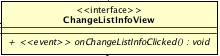
\includegraphics[scale=0.5]{Sezioni/SottosezioniST/img/app/ChangeListInfoView.png}
	\caption{feature::change\_list\_info::ChangeListInfoView}
\end{figure}

\begin{itemize}
\item \textbf{Descrizione}: Interfaccia che, una volta implementata, permette al presenter e allo sviluppatore di modificare la view dedicata alla modifica delle informazioni di una lista.
\item \textbf{Utilizzo}: L'interfaccia viene utilizzata per disaccoppiare presenter e implementazione della vista, e visualizza i dati che gli vengono passati dal presenter.
\item \textbf{Attributi}: 
\item \textbf{Metodi}:
\item{Eventi}:
	\begin{itemize}	
	\item \textit{public onChangeListInfoClicked():void}\\
		Evento che notifica tutti gli oggetti in ascolto che è stato cliccato il pulsante relativo alla modifica della lista.
	\end{itemize}
\end{itemize}

\subsubsection{feature::change\_list\_info::view::ChangeListInfoViewImpl}

\label{feature::change_list_info::view::ChangeListInfoViewImpl}
\begin{figure}[H]
	\centering
	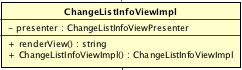
\includegraphics[scale=0.5]{Sezioni/SottosezioniST/img/app/ChangeListInfoViewImpl.png}
	\caption{feature::change\_list\_info::view::ChangeListInfoViewImpl}
\end{figure}

\begin{itemize}
\item \textbf{Descrizione}: Classe dedicata alla modifica dei dati e informazioni relativi alla lista.
\item \textbf{Utilizzo}: Il presenter fa da tramite tra l'implementazione della view e la parte logica dell'applicazione, formattando i dati che verranno visualizzati nella view e manipolando gli input dell'utente per eseguire le operazioni predisposte.
\item \textbf{Attributi}: 
	\begin{itemize}
	\item \textit{private presenter:ChangeListInfoViewPresenter}\\
	Il presenter associato alla view dedicata alla modifica dei dati relativi alla lista, al quale questa classe delega la gestione del comportamento della view stessa.
	\end{itemize}
\item \textbf{Metodi}:
	\begin{itemize}
	\item \textit{public ChangeListInfoViewImpl():ChangeListInfoViewImpl}\\
	Il costruttore della classe ChangeListInfoViewImpl.	
	\item \textit{public renderView():string}\\
	Genera il codice HTML CSS JS necessario per visualizzare la view.
	\end{itemize}
\item{Eventi}:
\end{itemize}

\subsubsection{feature::change\_list\_info::presenter::ChangeListInfoViewPresenter}

\label{feature::change_list_info::presenter::ChangeListInfoViewPresenter}
\begin{figure}[H]
	\centering
	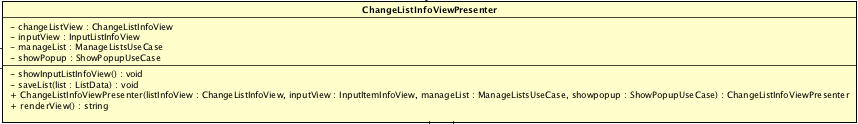
\includegraphics[scale=0.5]{Sezioni/SottosezioniST/img/app/ChangeListInfoViewPresenter.png}
	\caption{feature::change\_list\_info::presenter::ChangeListInfoViewPresenter}
\end{figure}

\begin{itemize}
\item \textbf{Descrizione}: Classe che rappresenta il presenter dedicato alla modifica delle informazioni di una lista.
\item \textbf{Utilizzo}: Il presenter fa da tramite tra l'implementazione della view e la parte logica dell'applicazione, formattando i dati che verranno visualizzati nella view e manipolando gli input dell'utente per eseguire le operazioni predisposte.
\item \textbf{Attributi}:
	\begin{itemize}
	\item \textit{private changeListView:ChangeListInfoView}\\
		La view associata al presenter.
	\item \textit{private inputView:InputListInfoView}\\
		Oggetto che rappresenta l'insieme dei dati immessi dall'utente durante la modifica della lista.
	\item \textit{private manageList:ManageListsUseCase}\\
Oggetto dedicato alla gestione dei dati relativi alla lista all'interno del database.
	\item \textit{private showPopup:ShowPopupUseCase}\\
		Oggetto che permette la creazione di un popup per l'immissione dei dati della lista da creare.	
	\end{itemize} 
\item \textbf{Metodi}:
	\begin{itemize}
	\item \textit{public ChangeListInfoViewPresenter(listInfoView:ChangeListInfoView, inputView:InputItemInfoView, \\ manageList:ManageListsUseCase, showpopup:ShowPopupUseCase):ChangeListInfoViewPresenter}\\
Il costruttore della classe ChangeListInfoViewPresenter.
			\\ \textbf{Parametri}: \begin{itemize}
			\item \textit{listInfoView:ChangeListInfoView}\\
			La view necessaria alla costruzione del presenter.
			\item \textit{inputView:InputListInfoView}\\
			Oggetto che rappresenta la vista per l'immissione dei dati relativi ad una lista.
			\item \textit{manageList:ManageListsUseCase}\\
			Oggetto dedicato alla gestione delle liste all'interno del database.
			\item \textit{showpopup:ShowPopupUseCase}\\
			Oggetto che permette la creazione di un popup per l'immissione dei dati della lista da modificare.	
			\end{itemize} 
	\item \textit{private showInputListInfoView():void}\\
		Metodo che permette di visualizzare il popup che conterrà la vista dove l'utente modificherà i dati della lista.
	\item \textit{private createViewForListWithId(listId:string):void}\\
		Metodo che permette di creare la vista per la modifica dei dati di una lista precompilando i campi di input con i dati della lista con id dato.
			\\ \textbf{Parametri}: \begin{itemize}
			\item \textit{listId:string}\\
			Id della lista i quali dati verranno utilizzati per precompilare i campi di input della vista.
			\end{itemize} 
	\item \textit{public renderView():string}\\
	Genera il codice HTML CSS JS necessario per visualizzare la view.
	\end{itemize} 
\item{Eventi}:
\end{itemize} 
